% =============================================================================
% File      : ex_doc_2-31.tex -- example 2.31
% Author    : Jürgen Hackl <hackl.j@gmx.at>
% Creation  : 2019-08-14
% Time-stamp: <Wed 2019-08-14 17:06 juergen>
%
% Copyright (c) 2019 Jürgen Hackl <hackl.j@gmx.at>
% =============================================================================
\documentclass{standalone}
\usepackage{../../tikz-network}
\begin{document}
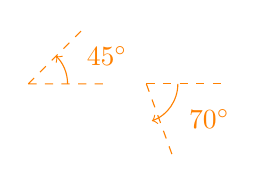
\begin{tikzpicture}
  \Vertex{A}
  \Vertex[x=1.5]{B}
  \Edge[loopposition=45](A)(A)
  \Edge[loopposition=-70](B)(B)
  \draw[orange,dashed](0,0) -- (10mm,0mm)(0,0)--(45:10mm);
  \draw[orange,->] (.5,0) arc (0:45:5mm);
  \node[orange] (x) at (1,.35) {$45^\circ$};
  \draw[orange,dashed](1.5,0)--++(-70:10mm);
  \draw[orange,dashed](1.5,0)--++(10mm,0);
  \draw[orange,->] (1.9,0) arc (0:-70:5mm);
  \node[orange] (x) at (2.3,-.45) {$70^\circ$};
\end{tikzpicture}
\end{document}
% =============================================================================
% eof

%%% Local Variables:
%%% mode: latex
%%% TeX-master: t
%%% End:
